%===================================== CHAP 4 =================================

\chapter{Research Method}\label{chap:4}

The purpose of this project is to create a prototype to improve students' motivation for applying for an exchange program by recommending courses and universities. The research questions were first created after defining the project's purpose and refined after identifying the background, motivation, relevant theory and related work through the preliminary research. The research questions were answered by evaluating a prototype created using the design and creation strategy. The final evaluation was done by using primarily quantitative data analysis on data generated by questionnaires and an offline experiment.

Oates'\cite{oates2005researching} model of the research process was used as a guideline for selecting the most appropriate research methods. The model and the specific methods chosen is displayed in Figure \ref{fig:research_process}. This chapter first presents the chosen research strategy. Next, the data generation methods and their respective data analysis methods are described. Lastly, the practical and ethical issues which influenced and limited the research project are discussed. 

\begin{figure}[H]
    \centering
    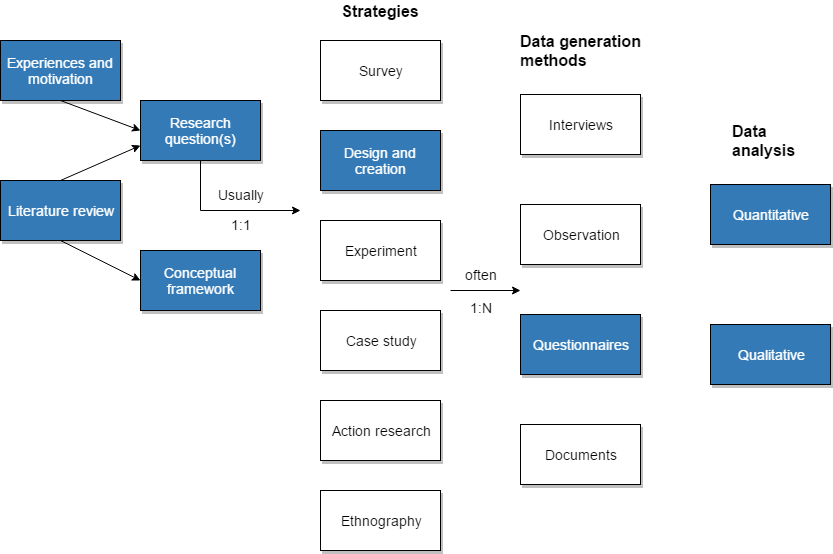
\includegraphics[width=1\textwidth]{fig/research_process.png}
    \caption[Research process]{Outlined research process for the project}
    \label{fig:research_process}
\end{figure}

\section{Research Strategy: Design and Creation}

The design and creation strategy focuses on creating computer-based artefacts which in some way contributes with new knowledge \cite{oates2005researching}. An artefact can be either be a contribution to new knowledge in itself, a tool used to answer questions, or the end-product of a development process focused project. This strategy adds research properties to regular software development by including academic qualities such as analysis, explanation, argument, justification and critical evaluation.

This project utilized the design and creation strategy to develop a prototype named Utsida. Utsida is an information system (IS) built from the identified system requirements (sec. \ref{sec:requirements}) and is used as a tool to answer both RQ1 and RQ2. The design and creation strategy follows the steps of the Design Science Research (DSR) process model defined by Vaishnavi and Kuechler \cite{vaishnavi2004design}. These steps are: Awareness, Suggestion, Development, Evaluation, and Conclusion.

\subsection{Awareness and Suggestion}
The awareness step involves finding and defining the problem domain, while in the suggestion step, the problem is refined into a tentative idea on how it might be solved. The domain was defined by the preliminary research (Ch. \ref{chap:2}), through the production of research questions (sec. \ref{RQ}) and by gaining knowledge on relevant theory (Ch. \ref{chap:3}). When the problem had been properly identified, a initial suggestion for the system was made. This suggestion included the first design details for the system which initiated the iterative development process.

\subsection{Development}

In the development step the idea formed in the suggestion step is implemented and a choice is made on what software development process to use. To answer the research questions it was necessary to produce data on user interaction and satisfaction. It was, therefore, essential that the web application part of Utsida was easy and intuitive to use. To ensure high user satisfaction, the software development of Utsida was done in an iterative process. This included communicating with potential users throughout the development and conducting usability tests. The spiral model, introduced by Boehm \cite{boehm1988spiral}, is a common model for iterative development, and was chosen as the foundation for the software development process of Utsida. Each spiral in the model includes steps for analyzing risks and requirements, development and testing of a prototype, planning the next iteration, and determining the objective of the next iteration. Figure \ref{fig:development_process} shows the chosen development process of Utsida. The process was inspired by the spiral model, but has less risk assessment, validation and planning. The changes were done to implement and test new functionality more rapidly. After each development step, the prototype was tested on students through usability tests. In the next step, verification and validation, the results of the usability tests were used to evaluate the prototype based on the requirements and goals. The development process was then continued if needed or terminated if the prototype was deemed ready for the final evaluation.

\begin{figure}[h]
    \centering
    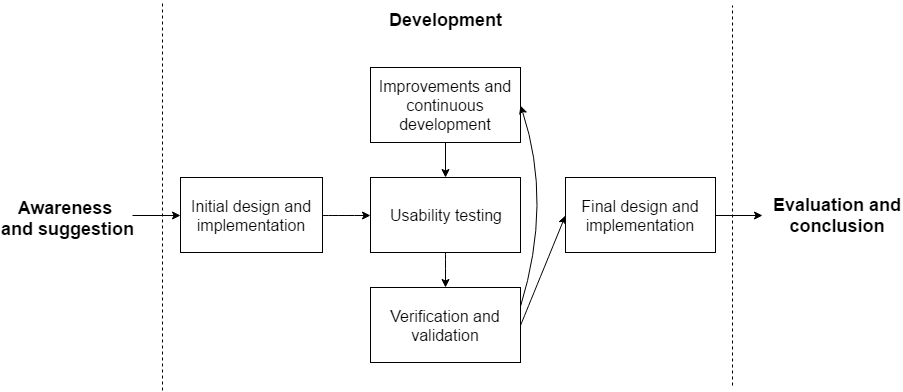
\includegraphics[width=1\textwidth]{fig/research_process_2.png}
    \caption[Development process]{Iterative development process of Utsida}
    \label{fig:development_process}
\end{figure}

\subsubsection{Usability Testing}

The usability tests in each development cycle were performed on the web application to evaluate and ensure sufficient usability. The test participants consisted in a large degree of students who had an understanding of the current approach for applying for an exchange program. Students from different study programs were tested to ensure a broad specter of backgrounds. These tests helped find and resolve flaws in both the general functionality and design so that the system was as reliable as possible before conducting the final user study. Data was collected by interviewing the testers, observing their use of the system, and have them fill out a System Usability Scale (SUS)-schema \cite{brooke1996sus}. During the interview the interviewee was asked questions such as \enquote{How would you expect this functionality to work?}, \enquote{Was it easy to navigate the system?} and \enquote{Was it intuitive to understand how that functionality works?}. After each test, the data was analyzed by using the SUS score \cite{brooke1996sus}.

\subsection{Evaluation and Conclusion}

In the evaluation step the developed prototype is assessed. The results and knowledge gained in the evaluation are then analyzed and discussed in the conclusion step. The final evaluation of Utsida and conclusion of the project was done by analyzing and discussing the data generated by the chosen data generation methods. Several methods were reviewed. Because there was no client, or persons with high stakes in this project, interviews were not viewed upon as a feasible method to generate data. Data generation through documents was also not a viable method, because of no existing documents about the problem context. The observation method was used in the usability tests but was not relevant for the final evaluation. However, questionnaires and experiments were suitable ways to generate data needed the answer the project's research questions and were, therefore, chosen as the methods to use. Using questionnaires made it possible to obtain generalized opinions on the system's motivational effect, and an experiment made it possible to objectively evaluate the suitability of the recommendations without user bias. Two questionnaires, questionnaire 1 and 2, and one experiment was used in the final evaluation. Questionnaire 1 was a study on motivational factors for going on exchange. Both questionnaire 2 and the experiment were designed after known methods of evaluating recommender systems, namely the user study and offline experiment methods introduced by Shani and Gunawardana \cite{shani2011evaluating}. The results of these data generations methods are presented in Chapter 6, and discussed in Chapter 7. 

\section{Questionnaires}

Questionnaire 1 (sec. \ref{sec:questionnaire_1}) was conducted during the development of the system with the goal of learning what students think are the most important motivational factors for choosing an exchange location. Questionnaire 2 (sec. \ref{sec:questionnaire_2}) was conducted after the prototype was deemed ready and was a final evaluation and user study of the prototype, Utsida.

Both questionnaires were self-administrated, which promoted the opportunity to collect data from a representative number of students at once. The target group of the questionnaires were students that had some experience with exchange studies. To acquire a large amount of students who were in this group, a cooperation with the OIR was made, and they agreed to publish the questionnaires on their Facebook page with approximately 3300 followers, most of them being in the target group of this research project.

In order to keep the margin of error to a minimum it was important to get feedback from as many students as possible. The target population of the questionnaires was students that have been on exchange from NTNU, and students that were interested in exchange. The population was roughly estimated to be between 10000 to 14000 students. According to Krejcie and Morgan \cite{krejcie1970determining} a sample size of approximately 370 is optimal (i.e. yield a margin of error less then 5\%) with a population size of 10 000. However, considering the limitations of budget, time and marketing resources, the expected sample size in this study was considerably lower than the optimal size. Hence, a sample size goal of 100 students was set for the questionnaires. With a population of 10 000 and confidence level of 95\% this would give a margin of error of approximately 10\% \cite{yamane1973statistics}. 

The majority of the questions in the questionnaires were closed questions formed as either: a Likert Scale \cite{allen2007likert}, a semantic differential scale \cite{osgood1952nature} or with \enquote{Yes}, \enquote{No}, or \enquote{Don't know} options. Also, the students were asked optional open questions where they could articulate their opinions. 

\subsection{Validity and Reliability}

Content validity is concerned with whether the questions in the questionnaire represents a good sample of the actual problem to be investigated \cite{oates2005researching}. This means that the selected questions should cover all the different evaluations needed to answer the research questions accurately. Feedback from potential participants and pilot tests were used to evaluate the validity, and the questions were formed with the possible evaluation criteria of the research questions in mind. For RQ1 the criteria is the use of the system and its motivational effect, while for RQ2, the criteria is if the system recommends viable universities and courses.

Construct validity means that the questionnaire is evaluating what it was intended to evaluate, and not other aspects \cite{oates2005researching}. Both questionnaires were designed to ensure the construct validity by using clear and straightforward questions that were in the scope of the research questions. The questionnaires were designed in an iterative process to remove or edit possible irrelevant or poorly formulated questions. 

The measurement of reliability measures whether the questionnaire yields consistent results. The reliability is difficult to assess in this study as the questionnaires were only published once, and they did not evaluate the system over time. Evaluating the prototype over time with part of the participants could also have distorted the data by giving them more time to be familiar with the prototype. However, one way to measure the reliability or internal consistency is using Cronbach's alpha \cite{bland1997statistics}, which was done on the Likert scale questions in questionnaire 2.

\subsection{Bias}

When using questionnaires as the primary method to collect data, several risks of bias can be introduced, including central tendency bias, acquiescence bias, social desirability bias and non-response bias \cite{furnham1986response}. This section presents these biases, how they could affect the results and how the risk of bias was reduced.  

\paragraph{Central tendency bias} is a risk when the questions have extreme response categories and is especially relevant for the Likert scale and Semantic Differential Scale. This bias means a participant is more likely answer in the middle of the scale. A lower point scale was used in questionnaire 2 to reduce the tendency of answers being in the middle of the scale. Both questionnaires also aimed to have clear questions that reduced the likelihood of participants to answer in the middle of the scale.

\paragraph{Acquiescence bias} is when the participant is likely to answer positively on a question \cite{cronbach1946response}. To reduce the acquiescence bias, the questions was designed to not be very positively based. However, due to the nature of the questions having less social desirability and not being of a sensitive type, an acquiescence bias was not likely to have a large impact. 

\paragraph{Social desirability bias} influence a participant to deny undesirable traits or positively answer questions that are socially desirable. Questions were striven to be neutral statements where the participants could state their degree of agreement. An example is the use of the Likert-type question format. 


\paragraph{Non-response bias} is when respondents' answers are considerably different from the possible answers of those that do not respond. Considering the response on the questionnaires was a small proportion of the full population, non-response bias was unavoidable. Those who did not participate might think the research sounds uninteresting, and if they participated, they might respond with more negative answers. Oppositely, the target population for the questionnaires were students who already had an interest in exchange studies, which might influence responses to be more positive. Non-response bias was taken into consideration in the discussion of the results.



\subsection{Questionnaire 1: Motivational Factors}\label{sec:questionnaire_1}

The goal of questionnaire 1 was to gain knowledge on important motivational factors for students when they choose an exchange location and university. The results from this questionnaire was also used to assign the weights of the attributes in the exchange experience concept, and used to justify what attributes to include. 

The main question in the questionnaire was closed and formed according to a seven-point semantic differential scale (see fig. \ref{fig:semantic_scale}). A seven-point scale was chosen to better fit the model in myCBR Workbench where the weights are represented in a range from 1-10. The participants ranked each motivational factor according to their opinion of the factor's decisiveness. Questionnaire 1 also included an open question which asked for input on other important motivational factors. See appendix \ref{app:questionnaire1_questions} for all the questions included in questionnaire 1. 

\begin{figure}[h!]
    \centering
    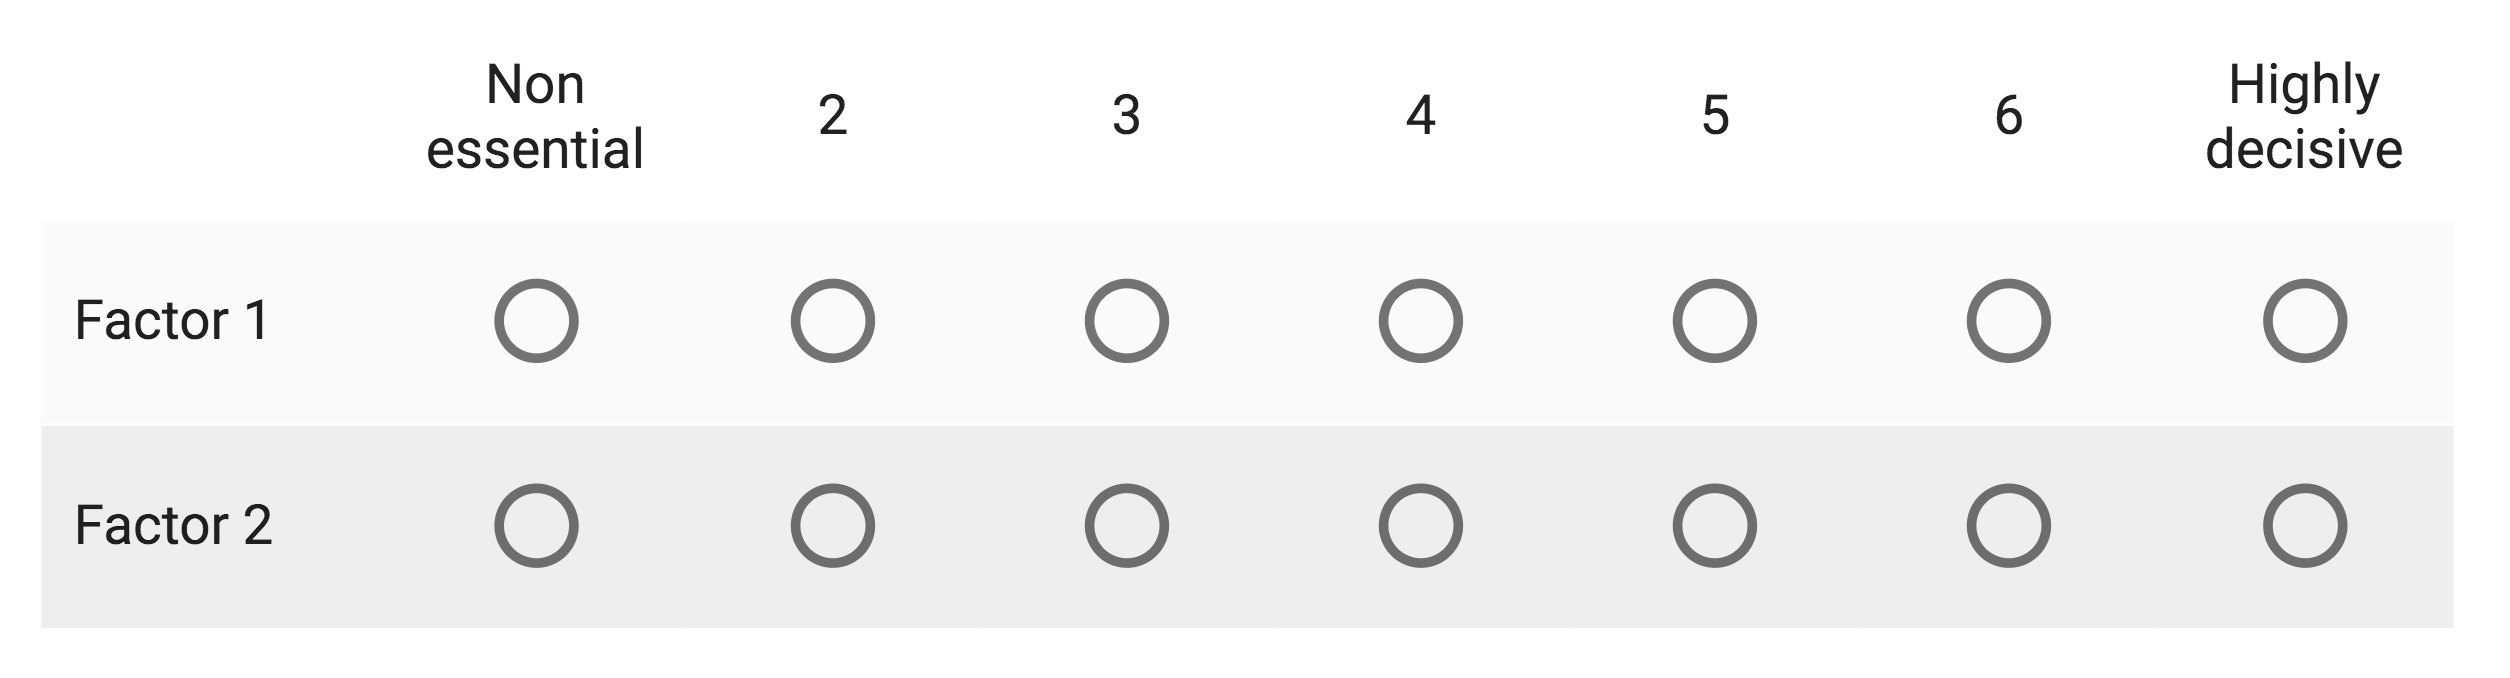
\includegraphics[width=1\textwidth]{fig/question1.png}
    \caption{Question format in questionnaire 1}
    \label{fig:semantic_scale}
\end{figure}

\subsubsection{Data analysis}

The numerical data from the questionnaire was analyzed in a quantitative manner, by calculating the mean, standard deviation and coefficient of variation for each attribute. The coefficient of variation (i.e. the spread relative to the mean of the data) was calculated to rank each attribute against each other. The resulting rank was then used to choose the weights of the attributes in the CBR-RS.

The open question was analyzed in a qualitative manner by using theme analysis \cite{oates2005researching}. Each answer was first reduced to only contain important sections related to the goal of the question. These important sections were then reduced to one or several common themes, and, finally, the number of occurrences of each theme was counted and ranked by importance.

\subsection{Questionnaire 2: User Testing of Utsida}\label{sec:questionnaire_2}

The three goals of questionnaire 2 was to: 1) evaluate and analyze how Utsida affects students' motivation for applying for an exchange program; 2) find out whether students who have already been on an exchange program thinks Utsida could have made their process easier; and 3) evaluate if Utsida gave relevant recommendations to the user.

The questionnaire was structured in two parts; one for reviewing the motivation and use of the application, and one for evaluating the CBR-RS' recommendations. All the questions from both parts can viewed in Appendix \ref{app:questionnaire2_questions}.

\subsubsection{Part 1: Motivational Effect and Use}
The goal of the questions in the first part was to find out what effect Utsida may have on the students motivation to apply for an exchange program (RQ1). The students were presented with slightly different questions depending on whether they had participated in an exchange program or not. The questions followed the Likert-type format \cite{likert1932technique} with a five-point scale where each option represents the degree of agreement to a given statement, shown in Figure \ref{fig:q2_question_form}

\begin{figure}[H]
    \centering
    
\includegraphics[width=1\textwidth]{fig/q2_question_form.PNG}
    \caption[Question format for selecting level of agreement on a statement]{Question format for selecting level of agreement on a statement in questionnaire 2}
    \label{fig:q2_question_form}
\end{figure}

\subsubsection{Part 2: Evaluation of Recommendations}

The second part of the questionnaire targeted RQ2 by letting students evaluate the recommendations they received from Utsida, and evaluate the recommendations from two pre-defined queries. The question form was designed to have simple \enquote{Yes}, \enquote{No}, \enquote{Don't know} answers to easier determine the amount of students that received relevant recommendations. The pre-defined queries (App. \ref{pre_defined_search_table}), were included to evaluate the recommendations for a specific query and to avoid the evaluations being affected by a participants' preference for a query. The evaluation of the pre-defined queries included a question which asked the students to rate the recommendations on a scale of suitability (Fig. \ref{fig:q2_rate_search}).

\begin{figure}[H]
    \centering
    
\includegraphics[width=1\textwidth]{fig/rate_search.png}
    \caption[Question format for evaluating suitability of recommendations]{Question format for evaluating suitability of recommendations for a pre-defined query in questionnaire 2}
    \label{fig:q2_rate_search}
\end{figure}


\subsubsection{Data Analysis}
The data analysis on the results from questionnaire 2 was done in a similar fashion as in questionnaire 1 by using quantitative analysis on the closed questions and simple qualitative analysis on the open question. The closed Likert-type questions produced ordinal data, meaning that the standard range between the values on the scale can not be determined. The data was, therefore, analyzed by using frequencies and mode. For the \enquote{Yes}, \enquote{No} or \enquote{Don't know} questions however, only percentages and number of answers for each option is used. Cronbach's alpha was used to asses the internal consistency of the Likert scale questions regarding motivation. 

\section{Offline Experiment on the CBR-RS}\label{sec:observation_test}

An offline experiment method introduced by Ricci et al. \cite{ricci2011introduction} was used to evaluate the relevancy of the recommendations of the CBR-RS, and thus contributed to answering RQ2. The experiment is a specific method to evaluate recommendation systems in an offline setting without user influence, and should not be misinterpreted as the \textit{Experiment} research strategy.

The offline experiment was conducted with 20 queries (App. \ref{app:user_queries}) that were generated to simulate 20 unique users. Each query was sent to two different concept configurations in the CBR-RS. One with adjusted similarity measures, taxonomies and weights, and one simulating standard exact match search. The simulation was done by only using exact match similarity measures and equal attribute weights. The scores for each recommendation was then given according to the score metric in Table \ref{tab:offline_test}, and the total score for each configuration was the mean score of each query. The hypothesis was that the configuration with adjusted similarity measures and weights would score higher than the configuration with a standard exact match search. 

This method made it possible to test the CBR-RS with a large set of inputs at a low cost. One downside of the method is that the queries only represent a small part of the possible user searches. This was mitigated by selecting a wide range of possible attributes and users profiles. Another disadvantage was that the offline experiment did not evaluate the CBR-RS with actual users, but it was mitigated by conducting continuous usability tests in addition to the user study with questionnaire 2. The Course attribute is not included in this experiment because the relevancy of the attribute is difficult to objectively measure and score without user feedback.


\begin{table}[h]
\centering
\resizebox{\textwidth}{!}{%
\begin{tabular}{|
>{\columncolor[HTML]{D0E0E3}}l |l|l|l|}
\hline
\multicolumn{4}{|c|}{\cellcolor[HTML]{A4C2F4}{\color[HTML]{333333} Rating scale for recommendations (0-10 points)}}                                                                                             \\ \hline
Attribute           & \cellcolor[HTML]{D0E0E3}0 points                                         & \cellcolor[HTML]{D0E0E3}1 point                                             & \cellcolor[HTML]{D0E0E3}2 points \\ \hline
Department           & \begin{tabular}[c]{@{}l@{}}Wrong faculty \\ wrong department\end{tabular} & \begin{tabular}[c]{@{}l@{}}Correct faculty\\ wrong department\end{tabular}   & Correct department                \\ \hline
Year                & Before 2011                                                              & 2011-2013                                                                   & 2014-2017                        \\ \hline
Geographic Location & \begin{tabular}[c]{@{}l@{}}Wrong country \\ wrong continent\end{tabular} & \begin{tabular}[c]{@{}l@{}}Correct continent\\ wrong country\end{tabular}   & Correct country                  \\ \hline
University          & \multicolumn{2}{c|}{No match}                                                                                                                          & Perfect match                    \\ \hline
Language            & No match                                                                 & \begin{tabular}[c]{@{}l@{}}The language is \\ part of the list\end{tabular} & Perfect match                    \\ \hline
Ratings             & \multicolumn{3}{c|}{0.5 points for each rating in range (-1, rating +1)}                                                                                                                  \\ \hline
\end{tabular}%
}
\caption[Score matrix for offline experiment]{Score matrix used to evaluate the recommendations in the offline experiment}
\label{tab:offline_test}
\end{table}

\subsection*{Data Analysis}
The offline experiment generated quantitative data that was statistically analyzed. The central tendency was analyzed with the mean and standard deviation measures, and a paired t-test was conducted to define the significance of the result. The confidence level of the t-test was 95\% with a p-value limit of 0.05.

\section{Ethical Issues}
Some ethical issues regarding data collection and storage were considered in project. The designated data collection methods kept all participants anonymous, but some meta-data was collected, such as which faculty and university they belong to. Furthermore, as an incentive for students to answer the questionnaires, lottery prizes were promoted for participating. To be able to enter the lottery, the participants had to enter their e-mail. The lottery was entirely optional and participants could register their answers without entering the lottery. The answers were stored in a Google Spreadsheet anonymously, and the entered e-mails were scrambled in a random order so that they were not linked to their answers. This way, there was no way to identify each answer. After the lottery was completed all the emails were deleted and only the winner contacted. 

Informed consent was maintained in the questionnaires by informing the participants about the purpose and goals for the questionnaires, and by stating that the entire process for all participants is entirely voluntarily and that they can stop any time they want.

During the online test of the system, the users created an account which included storing their chosen password, e-mail, name and department at NTNU. This information could not be linked to the questionnaire they took, but it still raised an ethical issue, considering the authors had access to this data. During the development of the system, steps were taken to ensure the confidentiality of the users of the system by using encryption and proper security measures.


\section{Practical Issues}
This study was performed by two students, with one supervisor to guide the project. There was a minuscule amount of monetary funds, and the available project duration was limited to nine months. The data which served as the results was primarily produced by real users. With the minimal budget, a practical issue was to produce incentive for enough students to answer the surveys. Furthermore, because of the limited time, both larger administrated tests and self-administrated tests were considered out of reach.

\cleardoublepage




